\documentclass[tikz,border=8pt]{standalone}
\usepackage{amsmath}
\usetikzlibrary{arrows.meta,positioning,fit,calc}

\begin{document}
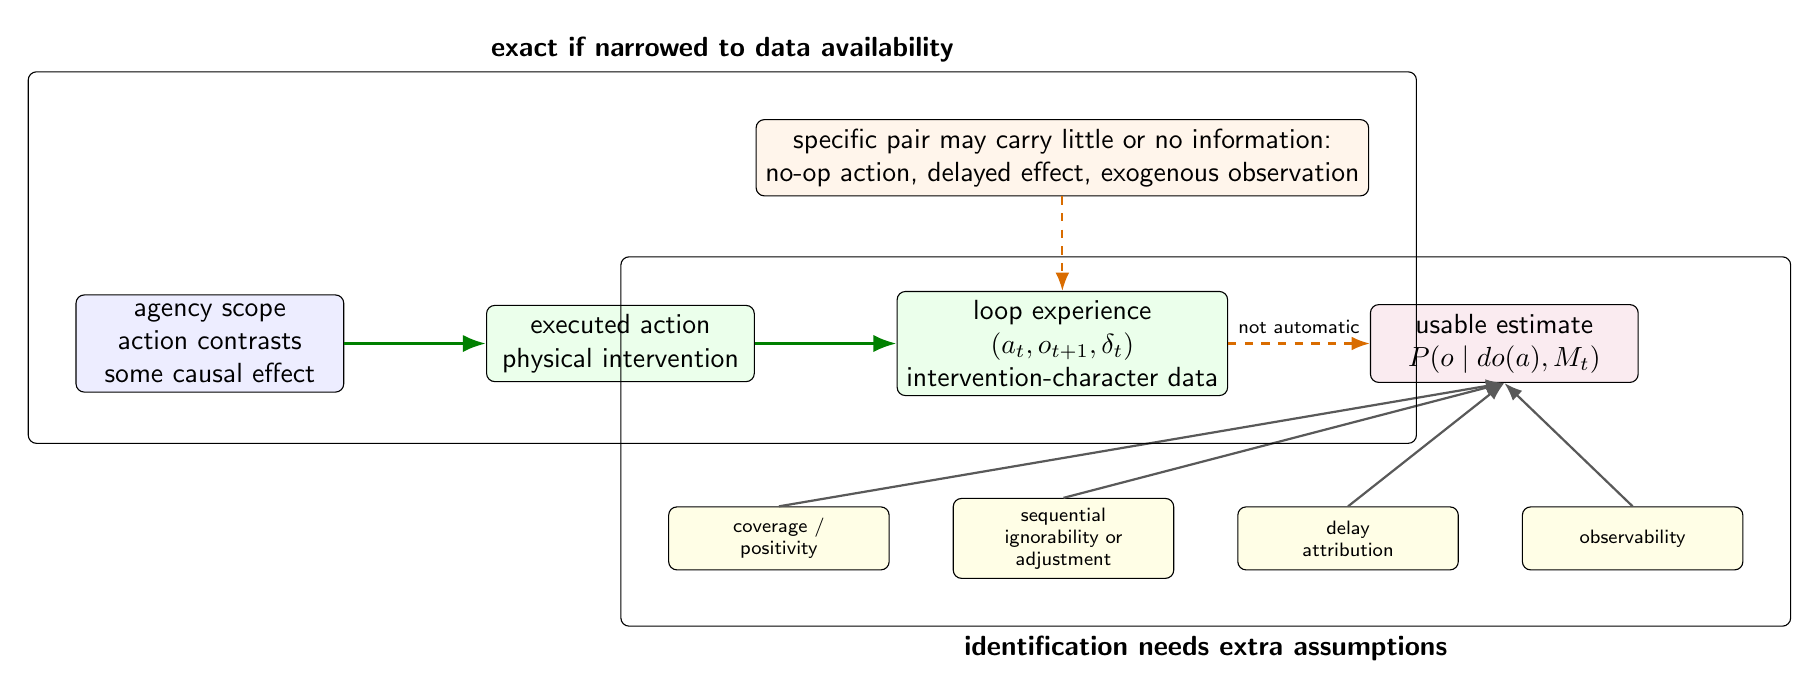
\begin{tikzpicture}[
  font=\sffamily,
  box/.style={draw, rounded corners=3pt, align=center, minimum width=34mm, minimum height=9mm, fill=white},
  gate/.style={draw, rounded corners=3pt, align=center, minimum width=28mm, minimum height=8mm, fill=yellow!10, font=\sffamily\scriptsize},
  arrow/.style={-Latex, thick, draw=black!65},
  good/.style={-Latex, very thick, draw=green!50!black},
  warn/.style={-Latex, thick, dashed, draw=orange!85!black},
  note/.style={align=center, font=\sffamily\scriptsize}
]

\node[box, fill=blue!7] (scope) {agency scope\\action contrasts\\some causal effect};
\node[box, right=18mm of scope, fill=green!8] (act) {executed action\\physical intervention};
\node[box, right=18mm of act, fill=green!8] (data) {loop experience\\$(a_t,o_{t+1},\delta_t)$\\intervention-character data};
\node[box, right=18mm of data, fill=purple!8] (identified) {usable estimate\\$P(o\mid do(a),M_t)$};

\draw[good] (scope) -- (act);
\draw[good] (act) -- (data);
\draw[warn] (data) -- node[above, note] {not automatic} (identified);

\node[gate, below=14mm of data, xshift=-36mm] (coverage) {coverage /\\positivity};
\node[gate, right=8mm of coverage] (ignorability) {sequential\\ignorability or\\adjustment};
\node[gate, right=8mm of ignorability] (delay) {delay\\attribution};
\node[gate, right=8mm of delay] (obs) {observability};

\foreach \g in {coverage,ignorability,delay,obs} {
  \draw[arrow] (\g.north) -- (identified.south);
}

\node[box, above=12mm of data, fill=orange!8, minimum width=45mm] (zero)
  {specific pair may carry little or no information:\\no-op action, delayed effect, exogenous observation};
\draw[warn] (zero) -- (data);

\node[draw, rounded corners=3pt, fit=(scope)(act)(data)(zero), inner sep=6mm,
  label={[font=\sffamily\bfseries]above:exact if narrowed to data availability}] {};
\node[draw, rounded corners=3pt, fit=(coverage)(ignorability)(delay)(obs)(identified), inner sep=6mm,
  label={[font=\sffamily\bfseries]below:identification needs extra assumptions}] {};

\end{tikzpicture}
\end{document}
